\documentclass{beamer}
\usepackage{xeCJK}

% Required packages
\usepackage{amsmath}
\usepackage{physics}
\usepackage{graphicx}
\usepackage{siunitx}
\usepackage{xcolor}
\usepackage{CJKutf8}

% Set image search paths
\graphicspath{{../images/}{../../shared/images/}}

% Define custom colors for DS9 theme
\definecolor{ds9blue}{RGB}{25,25,112}
\definecolor{ds9gold}{RGB}{218,165,32}
\definecolor{ds9grey}{RGB}{105,105,105}
\definecolor{ds9red}{RGB}{178,34,34}

% Set up the Madrid theme with custom colors
\usetheme{Madrid}
\usecolortheme{whale}

\setbeamercolor{palette primary}{bg=ds9blue,fg=white}
\setbeamercolor{palette secondary}{bg=ds9grey,fg=white}
\setbeamercolor{palette tertiary}{bg=ds9gold,fg=black}
\setbeamercolor{palette quaternary}{bg=ds9red,fg=white}
\setbeamercolor{structure}{fg=ds9blue}
\setbeamercolor{title}{fg=ds9gold}
\setbeamercolor{subtitle}{fg=ds9gold}
\setbeamercolor{frametitle}{bg=ds9blue,fg=white}
\setbeamercolor{block title}{bg=ds9blue,fg=white}
\setbeamercolor{block body}{bg=ds9grey!20,fg=black}

% Title page configuration
\title[电路学]{PHYS12 章节: 20, 21}
\subtitle{电路:原理、应用和安全}
\author[Gullo老师]{Gullo老师}
\date[2025年4月]{2025年4月8日}
\institute[物理系]{物理系}

\begin{document}

% Title page
\begin{frame}
    \titlepage
\end{frame}

% Table of contents
\begin{frame}
    \frametitle{课程概述}
    \tableofcontents
\end{frame}

% Learning objectives
\section{介绍}
\begin{frame}
    \frametitle{学习目标}
    \begin{block}{通过本课程,您将能够:}
        \begin{itemize}
            \item 定义电流、电阻和电压,并解释它们之间的关系
            \item 将欧姆定律应用于简单电路
            \item 计算串联和并联电路的等效电阻
            \item 计算电路中的电功率和能量
            \item 区分交流和直流电路及其特性
            \item 描述电气危害和生物电应用
            \item 解释测量仪器在直流电路中的工作原理
            \item 理解零位测量技术
            \item 描述RC电路在充电和放电过程中的行为
            \item 使用基尔霍夫定律解决复杂电路问题
        \end{itemize}
    \end{block}
\end{frame}

% Current and Ohm's Law section
\section{电流和欧姆定律}
\begin{frame}
    \frametitle{电流}
    \begin{block}{定义}
        电流是电荷流动的速率:
        \[ I = \frac{\Delta Q}{\Delta t} \]
        其中$\Delta Q$是在时间$\Delta t$内通过一个区域的电荷量。
    \end{block}
    \begin{itemize}
        \item 国际单位:安培(A),其中1 A = 1 C/s
        \item 传统电流:正电荷移动的方向
        \item 电流是自由电荷(电子、离子)的流动
        \item 与漂移速度相关:$I = nqAv_d$
    \end{itemize}
\end{frame}
\begin{frame}{}
    \begin{figure}
        \centering
        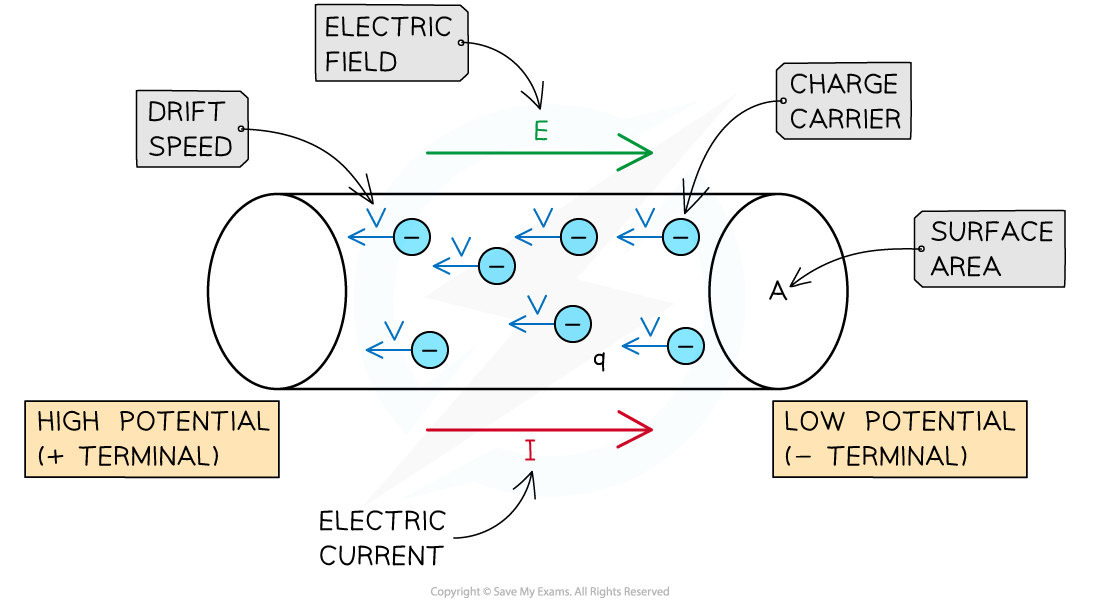
\includegraphics[width=1\linewidth]{phys12-circuits-charge-carrier-drift.png}
    \end{figure}
\end{frame}

\begin{frame}
    \frametitle{欧姆定律和简单电路}
    \begin{block}{欧姆定律}
        对于具有单一电压源和电阻的简单电路:
        \[ I = \frac{V}{R} \]
    \end{block}
    \begin{itemize}
        \item 电阻($R$):对电流流动的阻碍
        \item 单位:欧姆($\Omega$),其中1 $\Omega$ = 1 V/A
        \item 电阻器上的电压降:$V = IR$
    \end{itemize}
    \begin{center}
        \begin{figure}
            \centering
            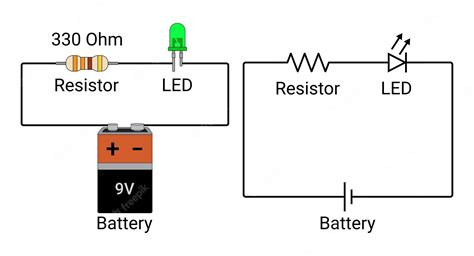
\includegraphics[width=0.5\linewidth]{phys12-gravity-newtons-law-of-universal-gravitation-formula.jpg}
        \end{figure}
    \end{center}
\end{frame}

\begin{frame}
    \frametitle{电阻和电阻率}
    \begin{block}{电阻公式}
        对于圆柱形导体:
        \[ R = \rho\frac{L}{A} \]
        其中$\rho$是电阻率,$L$是长度,$A$是横截面积。
    \end{block}
    \begin{itemize}
        \item 材料分类为导体、半导体或绝缘体
        \item 温度影响电阻率:$\rho = \rho_0(1 + \alpha\Delta T)$
        \item 温度影响电阻:$R = R_0(1 + \alpha\Delta T)$
        \item $\alpha$是电阻率的温度系数
    \end{itemize}
\end{frame}
\begin{frame}{}
    \begin{figure}
        \centering
        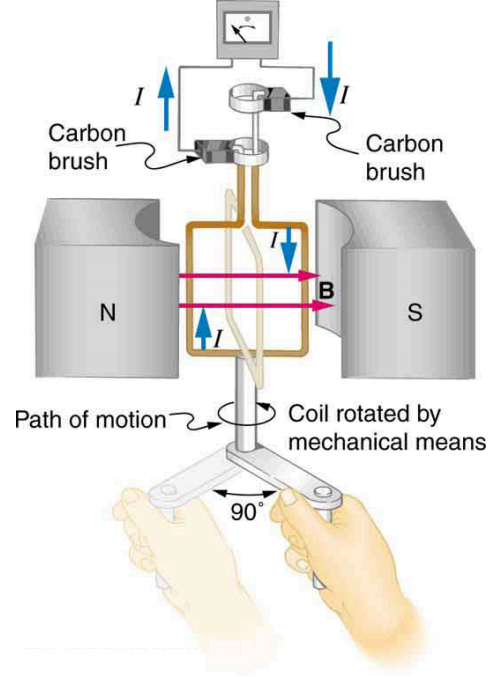
\includegraphics[width=1\linewidth]{phys12-circuits-rc-circuit-diagram.png}
    \end{figure}
\end{frame}

\begin{frame}
    \frametitle{电功率和能量}
    \begin{block}{电功率}
        电能被供应或消耗的速率:
        \[ P = IV = \frac{V^2}{R} = I^2R \]
    \end{block}
    \begin{itemize}
        \item 使用的能量:$E = Pt$
        \item 单位:瓦特(W)表示功率,焦耳(J)表示能量
        \item 示例:连接到120V的60W灯泡消耗0.5A电流
    \end{itemize}
    \vspace{0.5cm}
    \begin{alertblock}{功率比较}
        不同的功率额定值导致灯泡的不同亮度,
        电阻器产生的热量不同等。
    \end{alertblock}
\end{frame}

\begin{frame}
    \frametitle{交流电与直流电}
    \begin{block}{直流电(DC)}
        \begin{itemize}
            \item 电流仅在一个方向上流动
            \item 源电压恒定
            \item 示例:电池、太阳能电池、直流电源
        \end{itemize}
    \end{block}
    \begin{block}{交流电(AC)}
        \begin{itemize}
            \item 电压正弦变化:$V = V_0 \sin 2\pi ft$
            \item 电流正弦变化:$I = I_0 \sin 2\pi ft$
            \item $V_0$和$I_0$是峰值,$f$是以赫兹为单位的频率
            \item 示例:家用电、电力传输
        \end{itemize}
    \end{block}
\end{frame}

\begin{frame}
    \frametitle{交流电功率和有效值}
    \begin{block}{平均交流功率}
        \[ P_{ave} = \frac{1}{2}I_0V_0 = I_{rms}V_{rms} \]
    \end{block}
    \begin{itemize}
        \item 有效值(均方根):
        \[ I_{rms} = \frac{I_0}{\sqrt{2}} \quad \text{和} \quad V_{rms} = \frac{V_0}{\sqrt{2}} \]
        \item 交流电的欧姆定律:$I_{rms} = \frac{V_{rms}}{R}$
        \item 功率公式(类似于直流):
        \[ P_{ave} = I_{rms}V_{rms} = \frac{V_{rms}^2}{R} = I_{rms}^2R \]
    \end{itemize}
\end{frame}

\begin{frame}
    \begin{figure}
        \centering
        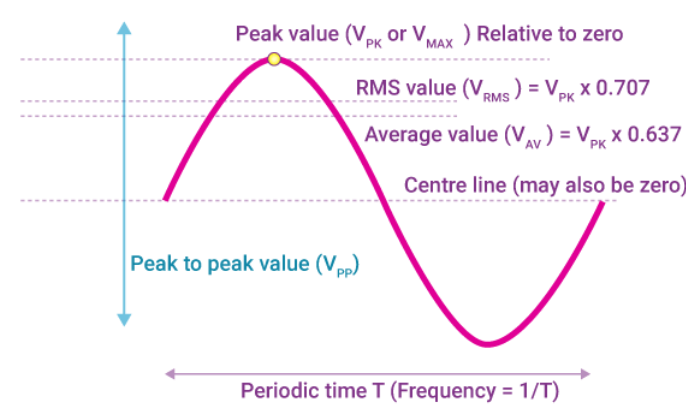
\includegraphics[width=0.75\linewidth]{phys12-circuits-rms-voltage-ac.png}
    \end{figure}
\end{frame}

\begin{frame}
    \frametitle{电气危害和人体}
    \begin{block}{电气危害类型}
        \begin{itemize}
            \item 热危害:过大功率导致烧伤或火灾
            \item 电击危害:电流流经人体
        \end{itemize}
    \end{block}
    \begin{block}{电击严重性因素}
        \begin{itemize}
            \item 电流大小
            \item 电流通过身体的路径
            \item 接触持续时间
            \item 交流电频率
        \end{itemize}
    \end{block}
    \begin{center}
        \begin{tabular}{|c|l|}
            \hline
            \textbf{电流(mA)} & \textbf{对人体的影响} \\
            \hline
            1 & 感知阈值 \\
            5 & 疼痛性电击,可引起肌肉收缩 \\
            10-20 & 无法松手,呼吸麻痹 \\
            100-300 & 心室颤动,可能导致死亡 \\
            \hline
        \end{tabular}
    \end{center}
\end{frame}

\begin{frame}
    \frametitle{神经传导和生物电}
    \begin{block}{生物电基础}
        \begin{itemize}
            \item 神经元中的电位差是由离子浓度差产生的
            \item 半透膜分隔不同的离子浓度
            \item 刺激改变膜的渗透性,产生动作电位
            \item 动作电位沿神经元传播,形成电信号
        \end{itemize}
    \end{block}
    \begin{block}{心电图(ECG)}
        \begin{itemize}
            \item 记录心脏的电活动
            \item 测量体表的电位差
            \item 有助于诊断心脏疾病和异常
        \end{itemize}
    \end{block}
\end{frame}
\begin{frame}{}
    \begin{figure}
        \centering
        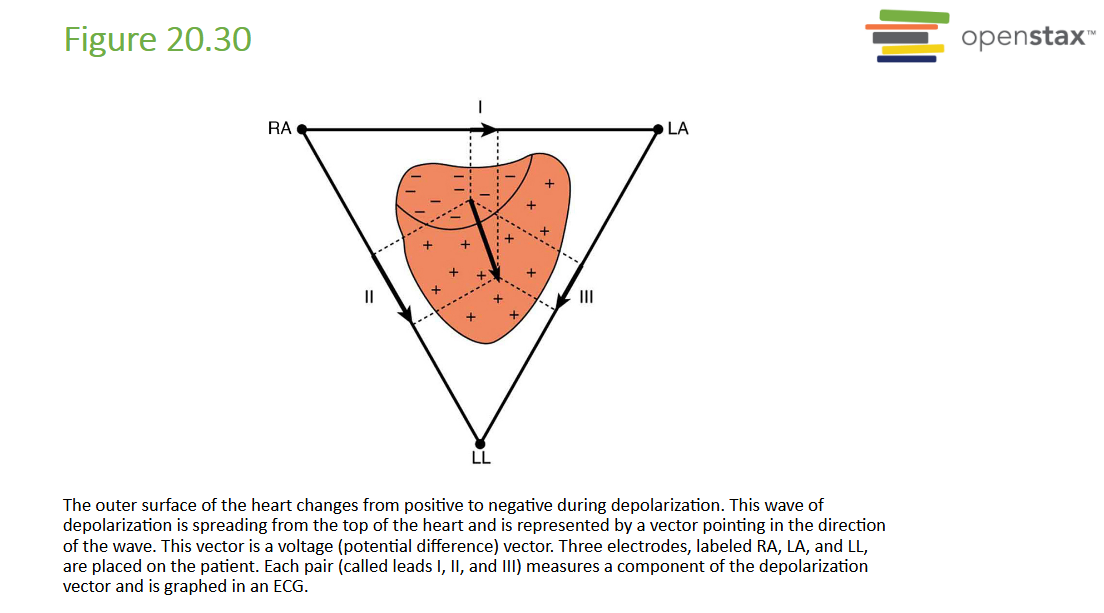
\includegraphics[width=1\linewidth]{phys12-circuits-ecg-waveform.png}
    \end{figure}
\end{frame}

% Complex Circuits section
\section{复杂电路}
\begin{frame}
    \frametitle{串联电阻}
    \begin{block}{串联配置}
        当电阻器首尾相连时,它们是串联的。
        \[ R_s = R_1 + R_2 + R_3 + \ldots \]
    \end{block}
    \begin{itemize}
        \item 相同的电流流过每个电阻器
        \item 电压在电阻器之间分配:$V = V_1 + V_2 + V_3 + \ldots$
        \item 单个电压降:$V_1 = IR_1$,$V_2 = IR_2$等
    \end{itemize}
    \begin{center}
        \begin{figure}
            \centering
            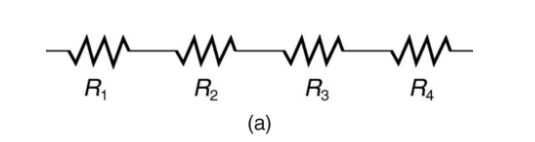
\includegraphics[width=0.75\linewidth]{phys12-circuits-resistors-in-series.png}
        \end{figure}
    \end{center}
\end{frame}

\begin{frame}
    \frametitle{并联电阻}
    \begin{block}{并联配置}
        当电阻器共享相同的两个端点时,它们是并联的。
        \[ \frac{1}{R_p} = \frac{1}{R_1} + \frac{1}{R_2} + \frac{1}{R_3} + \ldots \]
    \end{block}
    \begin{itemize}
        \item 每个电阻器上的电压相同
        \item 电流在电阻器之间分配:$I = I_1 + I_2 + I_3 + \ldots$
        \item 各个电流:$I_1 = \frac{V}{R_1}$,$I_2 = \frac{V}{R_2}$等
    \end{itemize}
    \begin{center}
        \begin{figure}
            \centering
            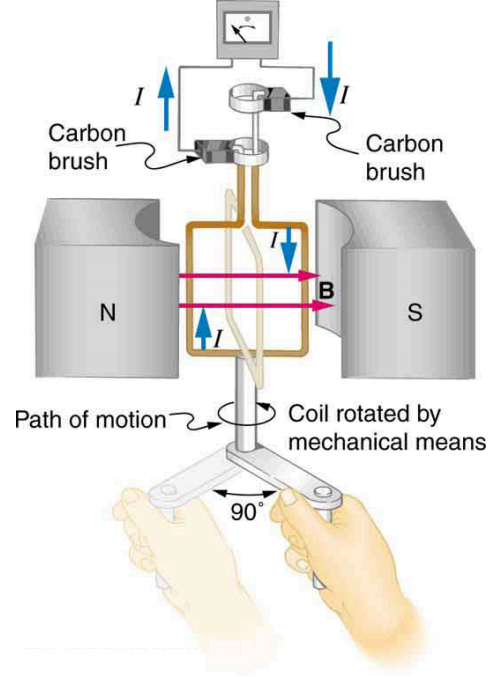
\includegraphics[width=0.5\linewidth]{phys12-circuits-rc-circuit-diagram.png}
        \end{figure}
    \end{center}
\end{frame}

\begin{frame}
    \frametitle{电动势和端电压}
    \begin{block}{电压源组成}
        实际电压源具有:
        \begin{itemize}
            \item 电动势(emf):没有电流流动时的电位差
            \item 内阻($r$):源内部的电阻
        \end{itemize}
    \end{block}
    \begin{itemize}
        \item 端电压:$V = \text{emf} - Ir$
        \item 串联电压源:内阻相加,电动势代数相加
        \item 太阳能电池:串联以增加电压,并联以增加电流
    \end{itemize}
\end{frame}
\begin{frame}
    \begin{figure}
        \centering
        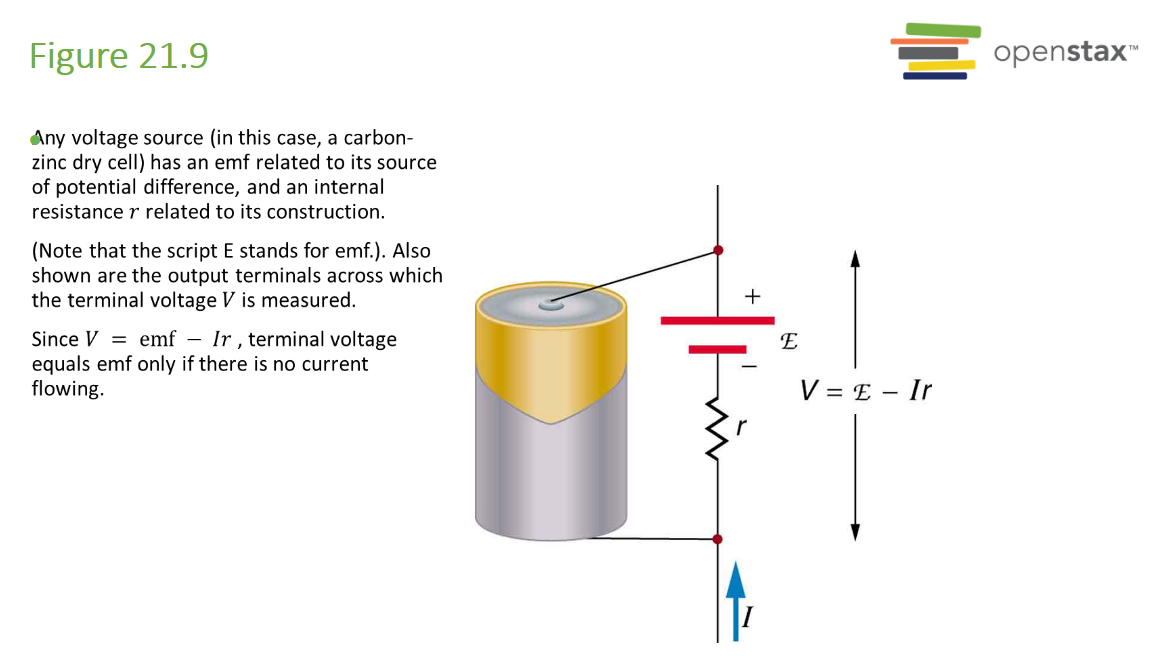
\includegraphics[width=1\linewidth]{phys12-circuits-internal-resistance.png}
    \end{figure}
\end{frame}
\begin{frame}
    \frametitle{基尔霍夫定律}
    \begin{block}{结点规则(第一定律)}
        流入结点的所有电流之和必须等于流出该结点的所有电流之和。
        \[ \sum I_{\text{in}} = \sum I_{\text{out}} \]
    \end{block}
    \begin{block}{回路规则(第二定律)}
        任何闭合电路路径(回路)上电位变化的代数和必须为零。
        \[ \sum \Delta V = 0 \]
    \end{block}
    \begin{itemize}
        \item 基于电荷和能量守恒
        \item 对分析复杂电路至关重要
    \end{itemize}
\end{frame}
\begin{frame}{}
    \begin{figure}
        \centering
        \includegraphics[width=1\linewidth]{junctionloopkirchov.jpg}
    \end{figure}
\end{frame}

\begin{frame}
    \frametitle{直流电压表和电流表}
    \begin{block}{测量仪器}
        \begin{itemize}
            \item 电压表测量电压(电位差)
            \item 电流表测量电流
        \end{itemize}
    \end{block}
    \begin{columns}
        \begin{column}{0.5\textwidth}
            \textbf{电压表特性:}
            \begin{itemize}
                \item 与组件并联连接
                \item 必须具有很高的电阻
                \item 最小化对电路的影响
            \end{itemize}
        \end{column}
        \begin{column}{0.5\textwidth}
            \textbf{电流表特性:}
            \begin{itemize}
                \item 与电路串联连接
                \item 必须具有很低的电阻
                \item 最小化电压降
            \end{itemize}
        \end{column}
    \end{columns}
    \begin{figure}
        \centering
        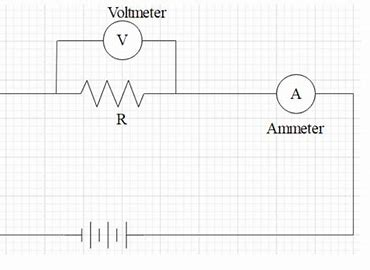
\includegraphics[width=0.3\linewidth]{phys12-circuits-ammeter-voltmeter-connection.jpg}
    \end{figure}
\end{frame}

\begin{frame}
    \frametitle{零位测量}
    \begin{block}{零位测量技术}
        \begin{itemize}
            \item 通过平衡电路实现更高的精度
            \item 在平衡点,没有电流流过测量设备
            \item 用于精确的电压和电阻测量
        \end{itemize}
    \end{block}
    \begin{columns}
        \begin{column}{0.5\textwidth}
            \textbf{电位计:}
            \begin{itemize}
                \item 精确确定电压
                \item 使用校准的可变电阻
                \item 将未知电压与已知电压平衡
            \end{itemize}
        \end{column}
        \begin{column}{0.5\textwidth}
            \textbf{惠斯通电桥:}
            \begin{itemize}
                \item 精确确定电阻
                \item 使用电阻比例
                \item 平衡时:$\frac{R_1}{R_2} = \frac{R_x}{R_3}$
            \end{itemize}
            \begin{figure}
                \centering
                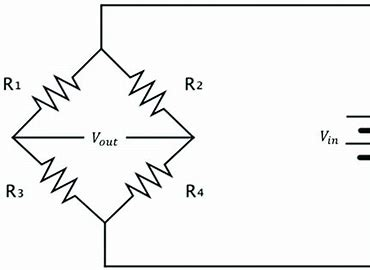
\includegraphics[width=0.5\linewidth]{phys12-circuits-wheatstone-bridge.jpg}
            \end{figure}
        \end{column}
    \end{columns}
\end{frame}

% RC Circuits section
\section{RC电路}
\begin{frame}
    \frametitle{RC电路基础}
    \begin{block}{RC电路定义}
        包含电阻器和电容器的电路。
    \end{block}
    \begin{itemize}
        \item 时间常数:$\tau = RC$
        \item 决定充电或放电的速率
        \item 单位:秒(s)
    \end{itemize}
    \begin{figure}
        \centering
        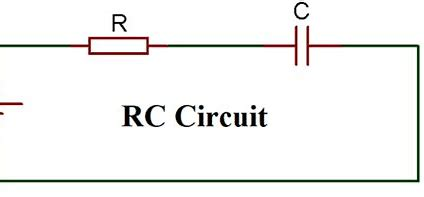
\includegraphics[width=0.65\linewidth]{phys12-circuits-kirchhoffs-junction-rule.jpg}
    \end{figure}
\end{frame}

\begin{frame}
    \frametitle{RC电路的充电和放电}
    \begin{block}{电容器充电}
        当初始未充电的电容器($t = 0$时$V_0 = 0$)被充电:
        \[ V = \text{emf}(1-e^{-t/RC}) \]
    \end{block}
    \begin{block}{电容器放电}
        当初始电压为$V_0$的电容器放电:
        \[ V = V_0e^{-t/RC} \]
    \end{block}
    \begin{itemize}
        \item 充电:每个时间常数电压上升剩余值的0.632
        \item 放电:每个时间常数电压下降剩余值的0.368
    \end{itemize}
\end{frame}

\begin{frame}
    \frametitle{RC电路:图形表示}
    \begin{center}
        \begin{tabular}{cc}
            \begin{figure}
                \centering
                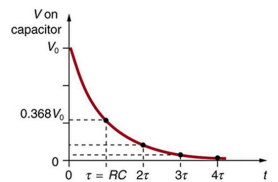
\includegraphics[width=0.5\linewidth]{phys12-circuits-capacitor-discharge-curve.png}
            \end{figure} 
            &
            \begin{figure}
                \centering
                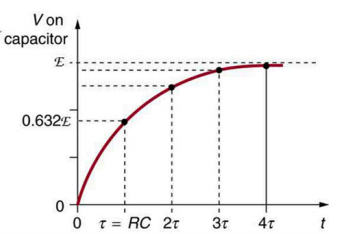
\includegraphics[width=0.4\linewidth]{phys12-electrostatics-charge-interactions.png}
            \end{figure} \\
            充电:$V = \text{emf}(1-e^{-t/RC})$ & 放电:$V = V_0e^{-t/RC}$
        \end{tabular}
    \end{center}
    \begin{itemize}
        \item 两个过程都是渐近的
        \item 理论上,完全充电/放电需要无限时间
        \item 实际上,经过5个时间常数后基本完成(99.99\%)
    \end{itemize}
\end{frame}

% Examples section
\section{例题}
\begin{frame}
    \frametitle{示范:等效电阻计算}
    \begin{block}{问题}
        计算具有三个电阻器的电路的等效电阻:$R_1 = 2.0~\Omega$和$R_2 = 4.0~\Omega$并联,$R_3 = 3.0~\Omega$与并联组合串联。
    \end{block}
    \begin{block}{解决方案}
        步骤1:计算$R_1$和$R_2$并联的等效电阻。
        \begin{align*}
            \frac{1}{R_p} &= \frac{1}{R_1} + \frac{1}{R_2} = \frac{1}{2.0~\Omega} + \frac{1}{4.0~\Omega}\\
            &= 0.5~\Omega^{-1} + 0.25~\Omega^{-1} = 0.75~\Omega^{-1}\\
            R_p &= \frac{1}{0.75~\Omega^{-1}} = 1.33~\Omega
        \end{align*}
        
        步骤2:通过将$R_p$和$R_3$串联相加来找到总电阻。
        \begin{align*}
            R_{total} &= R_p + R_3 = 1.33~\Omega + 3.0~\Omega = 4.33~\Omega
        \end{align*}
    \end{block}
\end{frame}

\begin{frame}
    \frametitle{共同练习:并联电路中的电流和功率}
    \begin{block}{问题}
        对于如图所示的电路,有一个12V电池,$R_1 = 4\Omega$和$R_2 = 8\Omega$并联,计算:
        \begin{enumerate}[(a)]
            \item 等效电阻
            \item 电池提供的总电流
            \item 通过每个电阻器的电流
            \item 每个电阻器上的电压
            \item 每个电阻器消耗的功率
        \end{enumerate}
    \end{block}
    \begin{figure}
        \centering
        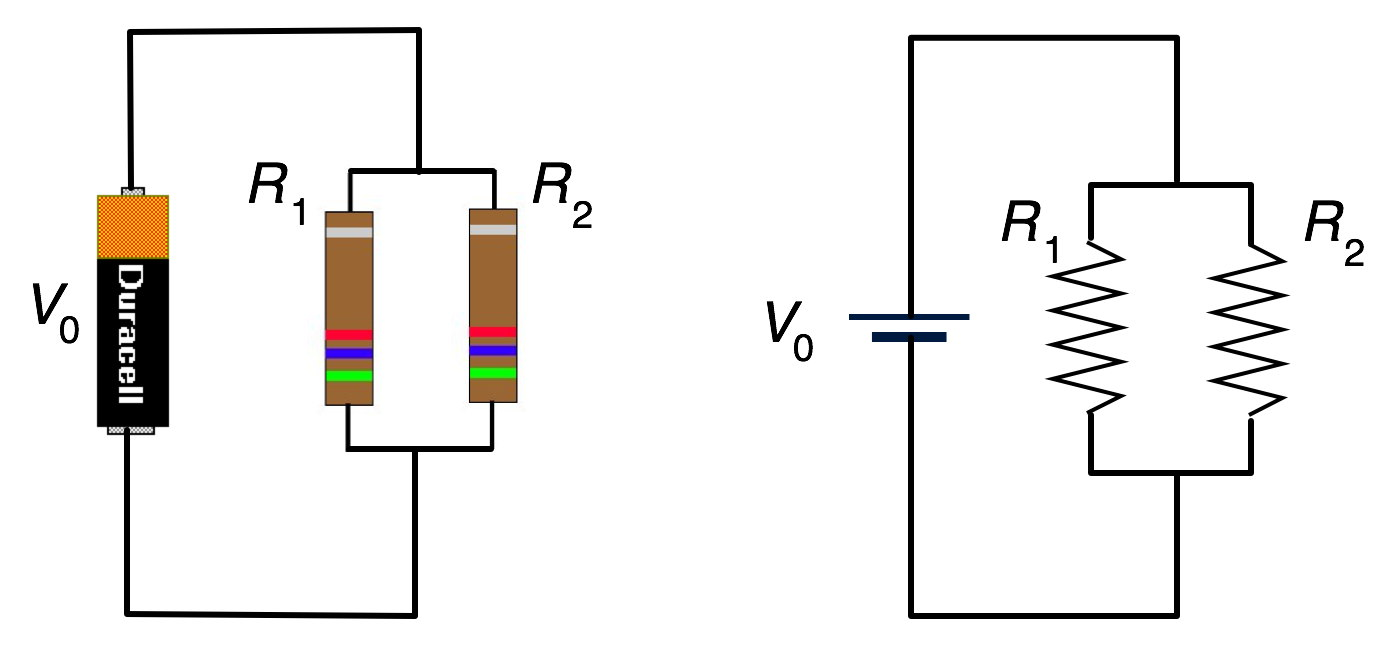
\includegraphics[width=0.5\linewidth]{phys12-circuits-parallel-circuit-with-battery.jpg}
    \end{figure}
\end{frame}

\begin{frame}
    \frametitle{共同练习:并联电路中的电流和功率}
    \begin{block}{部分解决方案}
        (a) 等效电阻:
        \begin{align*}
            \frac{1}{R_{eq}} &= \frac{1}{R_1} + \frac{1}{R_2} = \frac{1}{4\Omega} + \frac{1}{8\Omega}\\
            &= 0.25\Omega^{-1} + 0.125\Omega^{-1} = 0.375\Omega^{-1}\\
            R_{eq} &= \frac{1}{0.375\Omega^{-1}} = 2.67\Omega
        \end{align*}
        
        (b) 电池提供的总电流:
        \begin{align*}
            I_{total} &= \frac{V}{R_{eq}} = \frac{12V}{2.67\Omega} = 4.5A
        \end{align*}
        
        (c) 通过每个电阻器的电流:
        \begin{align*}
            I_1 &= \frac{V}{R_1} = \frac{12V}{4\Omega} = 3A\\
            I_2 &= \text{?} \quad \text{(完成此步骤)}
        \end{align*}
    \end{block}
\end{frame}

\begin{frame}
    \frametitle{共同练习:并联电路中的电流和功率}
    \begin{block}{部分解决方案(续)}
        (d) 每个电阻器上的电压:
        \begin{align*}
            V_1 &= \text{?} \quad \text{(完成此步骤)}\\
            V_2 &= \text{?} \quad \text{(完成此步骤)}
        \end{align*}
        
        (e) 每个电阻器消耗的功率:
        \begin{align*}
            P_1 &= \text{?} \quad \text{(完成此步骤)}\\
            P_2 &= \text{?} \quad \text{(完成此步骤)}
        \end{align*}
    \end{block}
\end{frame}

\begin{frame}
    \frametitle{自行练习:端电压和功率}
    \begin{block}{问题}
        电路包含一个内阻为$r = 0.5\Omega$的9V电池连接到一个$R = 5.5\Omega$的电阻器。
        \begin{enumerate}[(a)]
            \item 计算端电压。
            \item 计算电路中的电流。
            \item 计算电阻器消耗的功率。
            \item 计算电池内阻消耗的功率。
            \item 计算电池电动势提供的功率。
        \end{enumerate}
    \end{block}
\end{frame}

% Summary section
\section{总结}
\begin{frame}
    \frametitle{关键方程}
    \begin{columns}
        \begin{column}{0.5\textwidth}
            \textbf{电流和电阻:}
            \begin{itemize}
                \item $I = \frac{\Delta Q}{\Delta t}$
                \item $I = \frac{V}{R}$(欧姆定律)
                \item $R = \rho\frac{L}{A}$
            \end{itemize}
            
            \textbf{功率和能量:}
            \begin{itemize}
                \item $P = IV = \frac{V^2}{R} = I^2R$
                \item $E = Pt$
            \end{itemize}
            
            \textbf{交流电路:}
            \begin{itemize}
                \item $V = V_0 \sin 2\pi ft$
                \item $I_{rms} = \frac{I_0}{\sqrt{2}}$
                \item $V_{rms} = \frac{V_0}{\sqrt{2}}$
            \end{itemize}
        \end{column}
        \begin{column}{0.5\textwidth}
            \textbf{电路分析:}
            \begin{itemize}
                \item $R_s = R_1 + R_2 + R_3 + \ldots$
                \item $\frac{1}{R_p} = \frac{1}{R_1} + \frac{1}{R_2} + \ldots$
                \item $V = \text{emf} - Ir$
                \item $\sum I_{\text{in}} = \sum I_{\text{out}}$
                \item $\sum \Delta V = 0$
            \end{itemize}
            
            \textbf{RC电路:}
            \begin{itemize}
                \item $\tau = RC$
                \item $V = \text{emf}(1-e^{-t/RC})$(充电)
                \item $V = V_0e^{-t/RC}$(放电)
            \end{itemize}
            
            \textbf{零位测量:}
            \begin{itemize}
                \item $\frac{R_1}{R_2} = \frac{R_x}{R_3}$(惠斯通电桥)
            \end{itemize}
        \end{column}
    \end{columns}
\end{frame}

\begin{frame}
    \frametitle{概念回顾}
    \begin{itemize}
        \item 电流是电荷流动的速率;电阻阻碍电流。
        \item 欧姆定律关联简单电路中的电流、电压和电阻。
        \item 功率测量电路中能量传输的速率。
        \item 直流提供恒定电压;交流电压随时间正弦变化。
        \item 串联电阻增加;并联电阻减少。
        \item 实际电压源具有内阻,影响端电压。
        \item 基尔霍夫定律利用守恒原理帮助分析复杂电路。
        \item 正确连接测量仪器对准确读数至关重要。
        \item 零位测量技术为精确测量提供更高的精度。
        \item RC电路表现出由时间常数$\tau$特征的指数充电和放电行为。
        \item 电气安全需要了解电流阈值和电击危害。
    \end{itemize}
\end{frame}

\begin{frame}
    \frametitle{问题?}
    \begin{center}
        \Large 感谢您的关注!
        
        \vspace{1cm}
        
        有任何问题吗?
    \end{center}
\end{frame}

\end{document}